\chapter{Introduction}

% Intro should be readable to a non expert

\section{Goal}

The goal of this thesis is to develop methods for studying and using the
computations happening within complex dynamical systems to construct learning algorithms that
use a limited amount of supervision. We break down this objective into the
following subgoals: (i) identify complex dynamical systems with the potential to
exhibit emergent open-ended growth of complexity and evolutionary-like
properties.
\begin{figure}[htbp]
  \centering
\begin{subfigure}[b]{.4\linewidth}
  \centering
  
\includegraphics[width=\linewidth]{figures/disord2.png}
  \caption{A disordered \acl{CA}.}
 \label{fig:disordered_sys}
\end{subfigure}
\hspace{30pt}
\begin{subfigure}[b]{.4\linewidth}
  \centering
  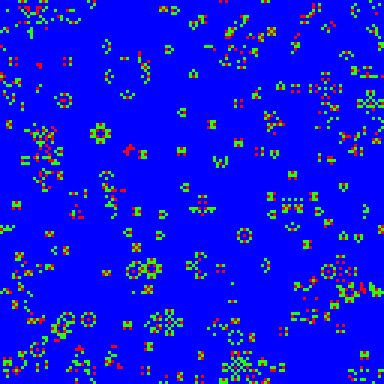
\includegraphics[width=\linewidth]{figures/micro4.png}
  \caption{A \acl{CA} with visible emergent structures.}
  \label{fig:structured_sys}
\end{subfigure}
\caption{Two example complex systems with different behavior types. Some
  \aclp{CA} appear more promising than others for the design of unsupervised
  learning systems because of their emergent complex structures (visible in \ref{fig:structured_sys}).}
  \label{fig:comparison_ca}
\end{figure}

(ii) Measure the fraction of systems that have the most complex and rapidly
evolving behavior. Defining these notions is also part of the goal. We believe
those systems to be the most promising for further use since they may exhibit
open-ended complexity growth.

\begin{figure}[htbp]
  \centering
 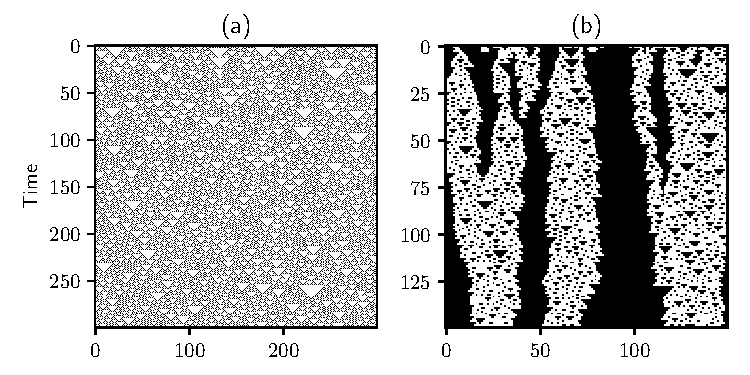
\includegraphics[width=.9\linewidth]{figures/rule18_small}
 \caption{Filtering the behavior of elementary \acl{CA} rule 18. This
   uncovers a highly structured behavior with the propagation of area boundaries
   within the apparent randomness.}
  \label{fig:rule_18}
\end{figure}


(iii) Apply promising systems to challenging tasks where classical machine
learning models may fail or prove less efficient. An example application is
illustrated in Figure~\ref{fig:ca_lm}, where a \ac{CA} is used to
implement a language model.

\begin{figure}[htbp]
  \centering
  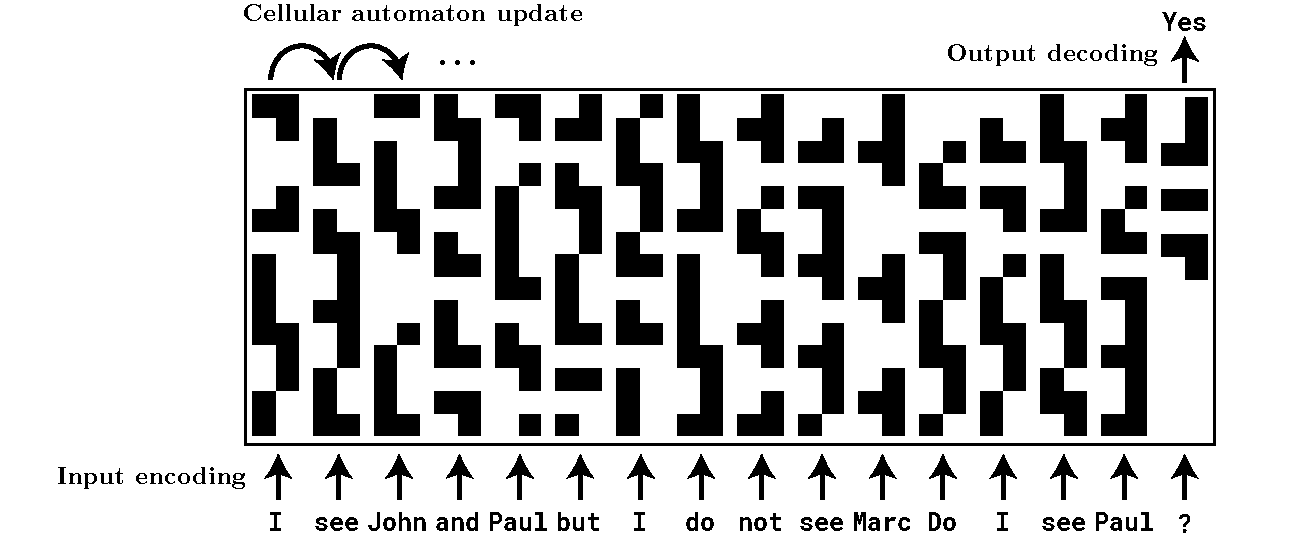
\includegraphics[width=.9\linewidth]{figures/ca_lm}
  \caption{An example of using a \acl{CA} and reservoir computing to implement a
    language model. Tokens are encoded within the \acl{CA} internal state. The
    \acl{CA} update rule is then applied and an output value is decoded from the
    final state.}
  \label{fig:ca_lm}
\end{figure}


In this work, we do not focus our attention on what the machine learning
community commonly refers to as ``unsupervised learning'', that is, learning
from untagged data. In machine learning, supervision refers to a label, a number,
or collection of numbers that represents the expected outcome of some input
data. Since our goal is to construct models that develop autonomously, we first
seek systems that behave this way, and postponing the issue of learning to
optimize a particular objective function.

In this thesis, we work toward achieving these goals, focusing on one particular
complex system: the \acl{CA}. This model has been extensively studied because of its simple definition and surprisingly complex behavior. We provide a
more precise definition of \aclp{CA} in Section \ref{sec:cellular-automata-sec}.


\section{Motivation}

Most of existing machine learning algorithms rely on the choice of an objective
function: a clearly defined mapping from the current state and parameters of a
model to a real value, which indicates the performance of that model. The
function depends on the objective of the model. For a supervised learning
problem, we may count the number of misclassified objects or the distance between
the predictions and the expected results. Even in unsupervised learning, the family of
algorithms learning from untagged data, objectives are still used. For
example, the well-known K-means clustering algorithm minimizes the sum of square
distances to cluster centers.

This reliance on objective functions creates two main issues: (i) the objective
is not always clearly defined. For example, a satisfying objective function for
a walking robot could be to ``not fall when stepping through its surrounding
environment''. This function is impractical to define and will vary a lot
depending on the parameters of the environment. Furthermore, (ii) Using such
functions as goals can be counterproductive because, as many examples in nature
demonstrate, the paths to these objectives are often deceptive. They involve
developing in unexpected directions that may initially seem against the original
goal \parencite{stanleyWhyGreatnessCannot2015}.

In this thesis, the term \emph{unsupervised} refers to a form of learning with
no predefined objective. Like natural evolution, we expect unsupervised
algorithms to develop new features autonomously and become progressively more
complex over time. Such algorithms would regularly learn to solve problems on
their own without the need to explicitly guide them, thereby discovering robust
and diverse solutions to deceptive problems.


\section{Challenges}

\begin{figure}[htbp]
  \centering
  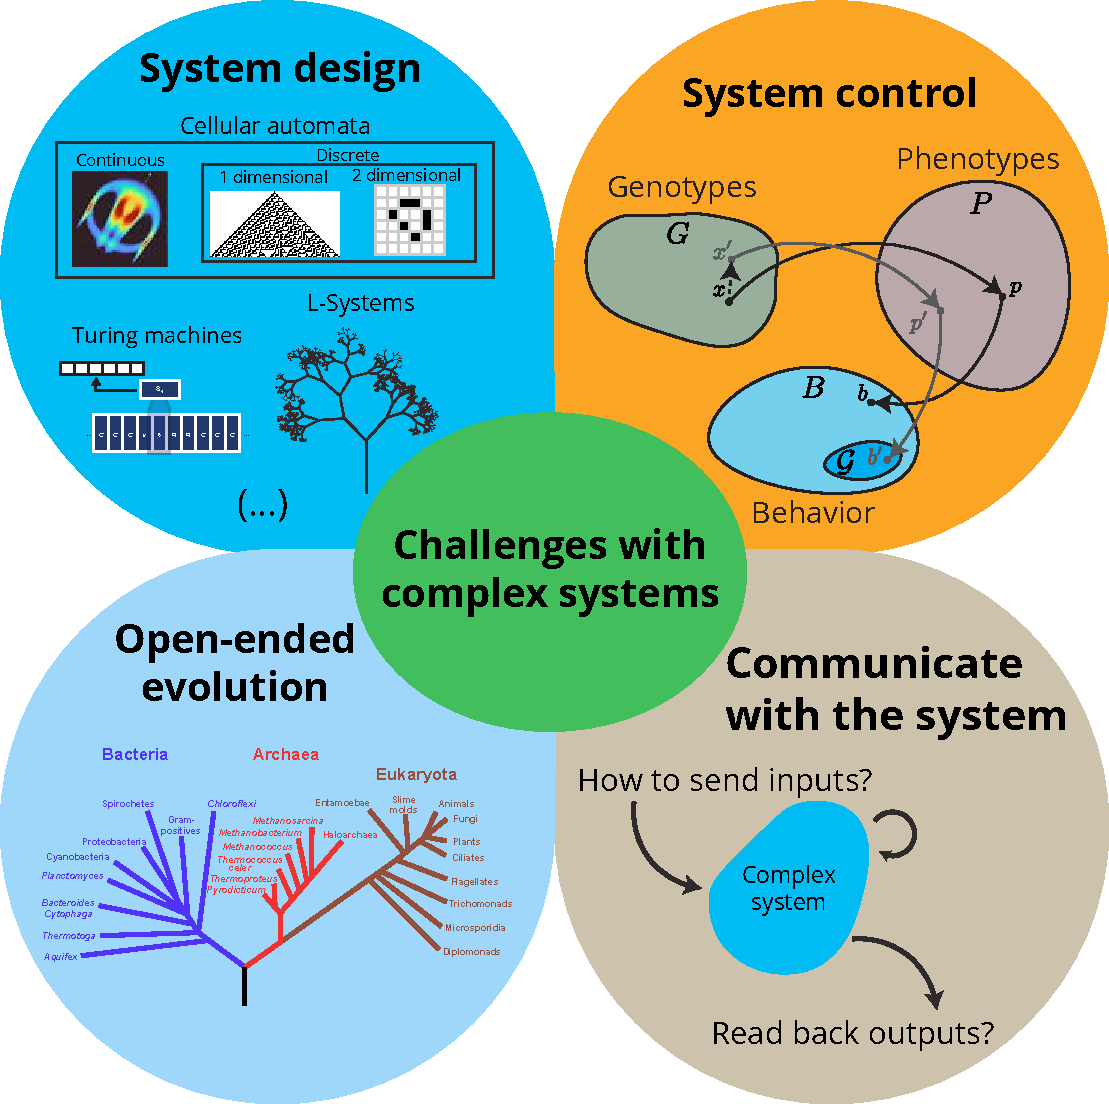
\includegraphics[width=.9\linewidth]{figures/challenges}
  \caption{The challenges of working with complex systems encountered across
    this thesis can be broken down in several categories. (top-left) The choice
    and design of the system, (top-right) the control of the system, the search
    for open-ended evolution properties, (bottom-left) the issue of sending
    inputs and (bottom-right) reading outputs from the internal state of a
    complex system.}
  \label{fig:challenges}
\end{figure}

The study of complex systems poses a range of difficult challenges in and of
itself \parencite{sanmiguelChallengesComplexSystems2012}. The complexity of a system
is an emergent property that arises from its intricate structure, its number of
elements, how it functions, and how it responds to different kinds of external
influence. For many complex systems, emergent mechanisms are poorly
understood.


\subsection{Design of a complex system}

The definition of complex systems is general, and several systems with
interesting dynamics can be studied. For example, L-Systems, Random Boolean
networks, Turing machines, and \Acfp{CA}. In the thesis, we focus mainly on
the latter: \ac{CA}. There are multiple benefits to working with this model. It
is very simply defined, and its high parallelism makes its implementation .

Choosing the right complex system architecture is essential because it defines
the search space over which interesting and useful systems can be found.
Correctly parametrizing that space can also be challenging, because too many
degrees of freedom make it difficult to find good systems, while too few might
indicate a lack of expressivity. An example parametrization of \ac{CA} with
little expressivity is Langton's lambda parameter
\parencite{langton_computation_1990}. On the other end of the spectrum, the
\ac{CA} rule is a simple parametrization with many degrees of freedom, which makes it
impractical.

Even when we limit ourselves to the study of \ac{CA}, many variants
can be considered. Cellular automata can have continuous or discrete states and operate in continuous or discrete space. For discrete state and space cellular
automata, the number of states and window of the update function can vary, as
well as the topology of the discrete space.


\subsection{Complex systems control}\label{sec:compl-syst-contr}

Many complex systems are chaotic. A deterministic dynamical system is said to be
chaotic if its evolution is highly sensitive to its initial conditions. Because
of this property, it is often very hard to predict how a given system will
evolve over time, and therefore hard to steer its evolution towards a particular
final state or along a chosen trajectory. This is an advantage for creating
open-ended systems, but it can make it challenging to apply these systems to some
basic tasks.

\subsection{Open-ended evolution without
  objectives}\label{sec:open-ended-evolution}

Another challenge is posed by the absence of a clear objective in the design of
unsupervised learning systems. Even without an objective, it is still essential
to understand which complex systems to choose from all available options or how
to tune them. This is why we need metrics that can help select interesting
systems without being another replacement objective function. The goal is to
make a system with the property of evolving in an open-ended way.

\subsection{Complex systems inputs and outputs}

Some of the complex systems we study in this thesis are closed systems. They do
not expect inputs or have well-defined outputs. Some examples of this
property are \ac{CA} and \ac{RBN}.

A common challenge for such
systems is to define the inputs and outputs in a way that preserves their internal
dynamics. This is also connected to the control problem of Section
\ref{sec:compl-syst-contr}, because controlling a complex system implies being
able to send a control signal and read back its current state.

Throughout this work, we use reservoir computing for this purpose.
Reservoir computing allows one to harvest the internal computations of complex
systems, or \emph{read} information from its internal state.


\section{Contributions}

The main contributions of this thesis are as follows,
\begin{enumerate}
  \item A thorough literature review that makes the connection between cellular
        automata and other complex systems literature and machine learning
        literature. Studying these two fields from a single point of view is
        relatively novel, and we consider a review necessary for placing the
        rest of our work in its context.

  \item The development of a general complexity metric that can help identify
        complex systems with interesting behavior.

  \item Development of a coarse-graining method to visualize computations
        in cellular automata and other discrete systems with local interactions.

  \item The introduction of a metric for learning efficiency for learning
        algorithms as well as a benchmark dataset of progressively harder
        language tasks.
\end{enumerate}

\section{Thesis overview}

In Chapter \ref{cha:literature-review}, we review relevant methods and tools for
measuring the complexity of complex systems and using their computations for
various tasks.

Chapter \ref{cha:background} presents some background notions about complex
systems, cellular automata, and reservoir computing.

Chapter \ref{cha:meas-compl-evolv} introduces a complexity metric that allows us 
to select complex systems with interesting behavior. The metric measures the
``novelty'' of the temporal states of a system compared to a reference one. We
built a dataset of interesting cellular automata to validate the quality of the
metric.

Chapter \ref{cha:visu-comp-large} addresses the question of large-scale complex
systems and the applicability of complexity metrics at multiple scales. We
propose three algorithms for the coarse-graining of cellular automata. This allows
us to reduce the size of large-scale systems while retaining the interesting parts
of the behavior.

Chapter \ref{cha:learn-effic-compl} presents a learning efficiency metric and a
dataset to measure the speed of learning of various systems. We show that
reservoir computing-based systems using cellular automata can be more efficient
than usual machine learning algorithms in constrained data and computation
settings.


\section{Publications and software}

The thesis has led to the following publications.

\begin{itemize}
  \item \fullcite{cisnerosEvolvingStructuresComplex2019}
  \item \fullcite{cisnerosVisualizingComputationLargescale2020}
  \item \fullcite{cisnerosBenchmarkingLearningEfficiency2022a}
\end{itemize}

The code to reproduce the experiments of all three publications is available on
GitHub.

We also published a dataset that we used for our benchmark in our last
publication. It is available at
\url{https://github.com/hugcis/incremental_tasks/}.
